\subsection{Grundlagen und Methode}
Im Rahmen der PeP et al. Sommerakademie 2013 wurde unter anderem das Projekt Astrofotografie durchgeführt. Ziel war es, verschiedene Bilder der Milchstraße, von Sternbildern und Deep-Space-Objekten zu erstellen.

Will man im Bild die einzelnen Sterne als solche erkennen, setzt die Erdrotation eine obere Schranke an die Belichtungszeit, die auch abhängig vom Bildwinkel bzw. der Brennweite des Objektivs ist. Im starken Weitwinkelbereich konnten Zeiten bis zu 15\,s verwendet werden, diese Zeit verkürzt sich dramatisch auf unter 3s, wenn man Brennweiten $>150$\,s verwendet.

Bei diesen Belichtungszeiten werden sehr starke Verstärkungen des Lichtsignals nötig (hoher ISO-Wert), dies führt zu einem recht starken Rauschen. Dies lässt sich reduzieren, indem man die Bilder mit entsprechender Software, verwendet wurde Fitsworks, zunächst ausrichtet und dann mittelt.

\subsection{Beispielbilder}

\begin{figure}[!h]
\centering
\includegraphics[width=\textwidth]{figs/astro/Haufen.jpg}
\caption{Aufnahme der Milchstraße, 50 Bilder gemittelt. 300mm, f:4,5, ISO 25600,  je 4s}
\end{figure}


\begin{figure}
\centering
\includegraphics[width=\textwidth]{figs/astro/Haufen_crop1.jpg}
\caption{Bildauschnitt aus oberem Bild, sichtbar zwei Sternhaufen innerhalb der Milchstraße}
\end{figure}


\begin{figure}
\centering
\includegraphics[width=\textwidth]{figs/astro/m101_add_50.jpg}
\caption{Aufnahme der Spiralgalaxie M101 im großen Wagen, sichtbar im oberen linken Bilddrittel 50 Bilder gemittelt. 300mm, f:4,5, ISO 25600, je 4s}
\end{figure}


\begin{figure}
\centering
\includegraphics[width=\textwidth]{figs/astro/m101_crop.jpg}
\caption{Bildauschnitt aus oberem Bild, die Spiralarme von M101 lassen sich deutlich erkennen}
\end{figure}


\begin{figure}
\centering
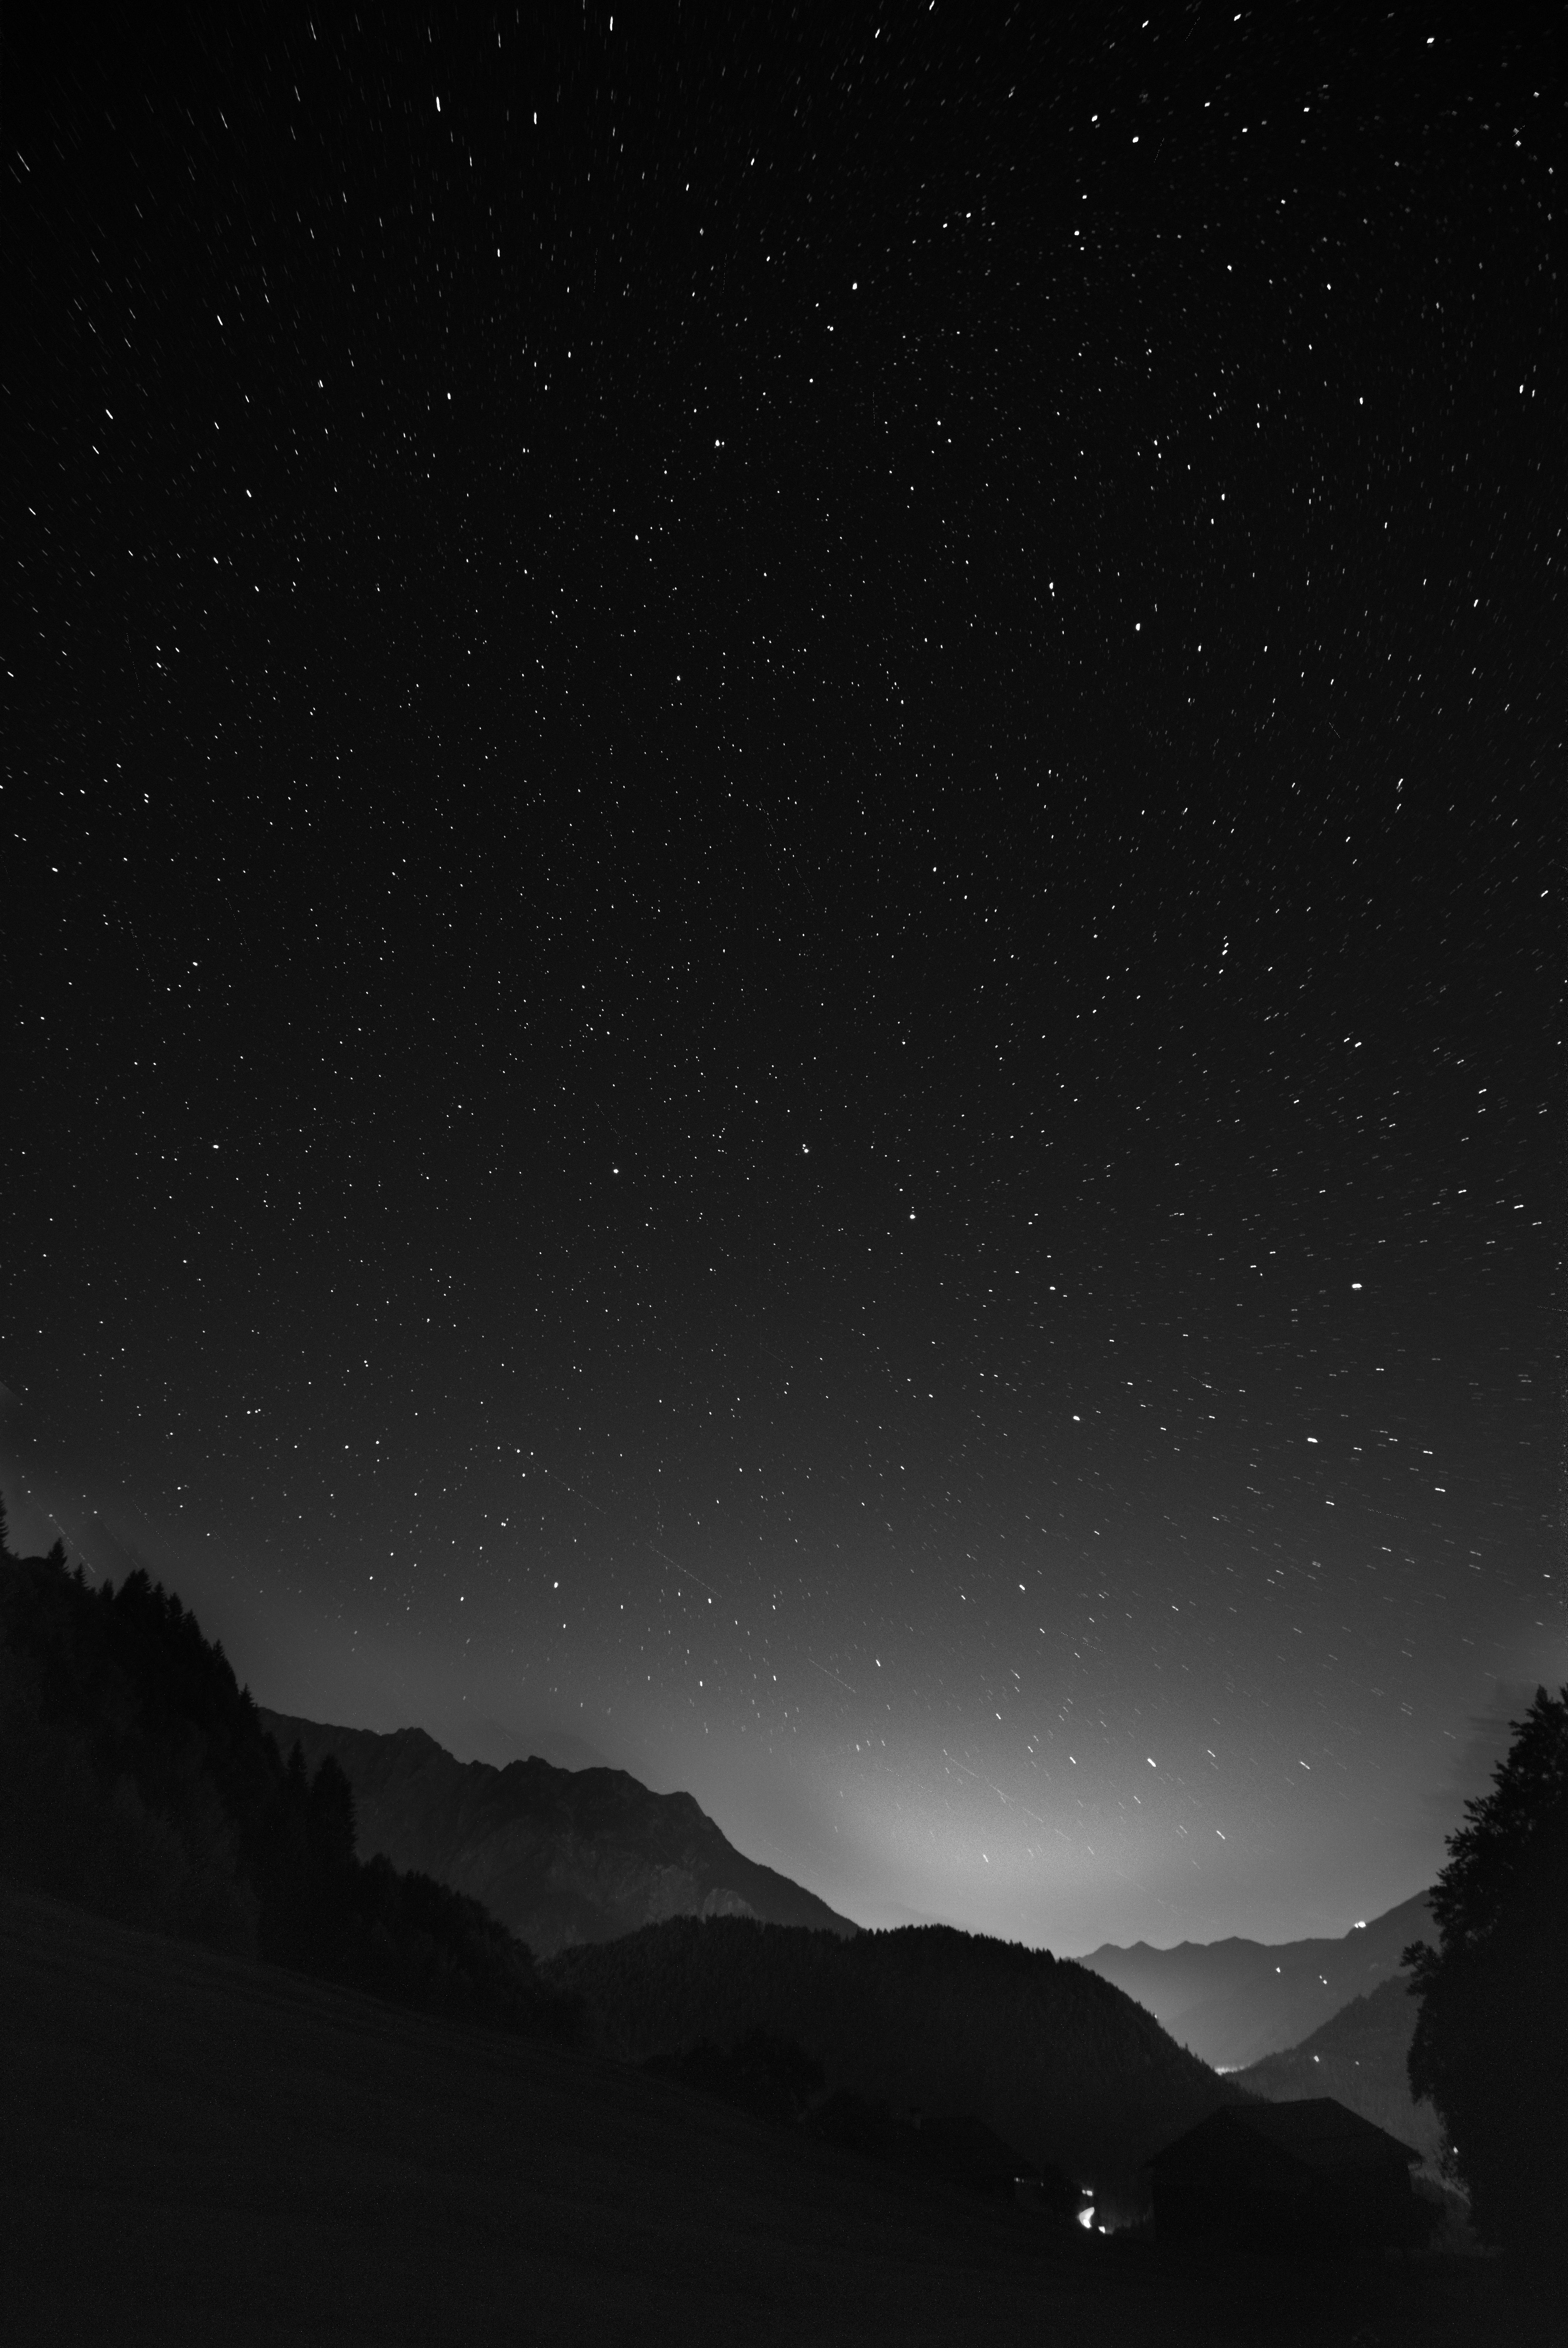
\includegraphics[width=\textwidth]{figs/astro/berg_wagen_2.png}
\caption{Aufnahme des Sternenhimmels mit großem Wagen, Kombination aus 17 Bildern, 16mm, 15s, f:2,8 ISO 1600, Gemittelt wurde einmal mit Nachführung für den Sternenhimmel und einmal ohne Nachführung für den Vordergrund  anschließend beide Bilder in Photoshop mit einer Ebenenmaske kombiniert}
\end{figure}